\scanpage{97}
application. On n'exige plus que $\sigma_{\unsure{\widehat I|\widehat A}}$ soit sans pts fixes — l'ens des pts fixes, $I$, \deleted{se} correspond aux ``branches orphelines'' du $1$-complexe i.e. aux \deleted{``\unsure{bouts}''} ``pts-bord'' de $X$ qui ne sont pas dans $S$. La donnée d'un graphe à branches orphelines revient donc (en décomposant $\widehat I$ en $I\amalg\widetilde A$, où $I=\widehat I^\sigma$ et $\widetilde A=\widehat I\setminus\unsure{\widehat I^\sigma|I}$) à la donnée d'un \deleted{couple} graphe ordinaire \inserted{$(S,\widetilde A,\sigma_{\widetilde A},o_{\widetilde A})$}, plus un ensemble $I$ et une application $I\longrightarrow S$.

On décrit un tel graphe à branches orphelines par un graphisme tel que
\figure{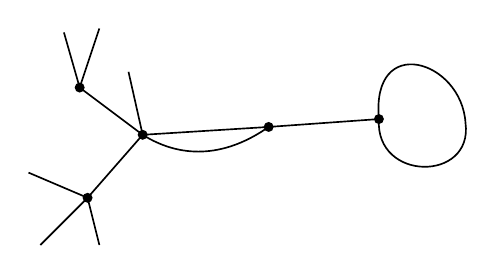
\begin{tikzpicture}[x=1cm,y=1cm,line width=.6pt]
\coordinate (a) at (0,0); \coordinate (b) at (-.8,.6); \coordinate (c) at (-.7,-.8); \coordinate (d) at (1.6,.1); \coordinate (e) at (3,.2);
\draw (a)--(b) (a)--(c) (a)--(d)--(e);
\draw (a) to[out=-32,in=-145] (d);
\draw (e) .. controls (2.9,1.3) and (4.05,.95) .. (4.1,.15) .. controls (4.2,-.6) and (2.95,-.6) .. (e);
\draw (b)--(-1,1.3) (b)--(-.55,1.35) (c)--(-1.45,-.48) (c)--(-1.3,-1.4) (c)--(-.55,-1.4) (a)--(-.18,.8);
\foreach \p in {a,b,c,d,e} {\fill (\p) circle (1.8pt);}
\end{tikzpicture}}
où les sommets sont figurés par des points gros $\bullet$, et les branches orphelines \deleted{sont} se distinguent par le fait justement qu'elles ne sont pas marquées \inserted{en} gros. Le graphe \inserted{à \unsure{b.o.|b.a.}} ci-dessus correspond donc, avec la notion des ``pieds marqués'', à
\figure{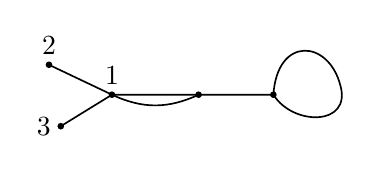
\begin{tikzpicture}[x=1cm,y=1cm,line width=.6pt]
\coordinate (a) at (0,0); \coordinate (b) at (-.8,.38); \coordinate (c) at (-.65,-.4); \coordinate (d) at (1.1,0); \coordinate (e) at (2.05,0);
\draw (b)--(a)--(c) (a)--(d)--(e);
\draw (a) to[out=-25,in=-155] (d);
\draw (e) .. controls (2.1,.75) and (2.75,.7) .. (2.9,.12) .. controls (3.05,-.4) and (2.3,-.4) .. (e);
\foreach \p in {a,b,c,d,e} {\fill (\p) circle (1.2pt);}
\node[above] at (a) {$1$}; \node[above] at (b) {$2$}; \node[left] at (c) {$3$};
\end{tikzpicture}}
\margin{96}
